\chapter{Concept}

This chapter outlines the impact of the study's findings and explains the rationale behind the method's design, considering both theoretical principles and practical evidence. 
We aim to manipulate the position of a person within a point cloud without physically relocating a real person. This process involves extracting the point cloud corresponding to a person by leveraging geometric characteristics of points in three-dimensional space, followed by transforming the person's point cloud to a specified location. This approach enables to evaluate the response of a 3D object detection model to different scenarios wherein the person is situated in varied locations or within distinct background point cloud scenarios.

In this project, we refer to the source scene cloud as the point cloud from where an object or prototype needs to be extracted. A prototype is an object or a part of the source scene cloud that represents the point cloud of an actual object or object of our interest (person). The target scene cloud is the cloud where we insert the extracted prototype cloud, creating a new scenario cloud. Generally, at a high level, the system consists of two major steps which consist of sub-steps. The first step is represented by prototype extraction, which is represented by green color in the figure \ref{fig:concept-graph}. In this step, the prototype is extracted from the source scene cloud. The second major step is called as recombining of points cloud that is represented by red color on the figure \ref{fig:concept-graph}. In this step, the prototype extracted from the source scene is merged or recombined with the target scene cloud. Further recalculation of the point cloud of the prototype and calculation of shadow casting on the target scene is done in this step. The result of the system is a target scene consisting of a prototype cloud that resembles as if there was an actual prototype object on the scene. In the following section, we discuss each step in detail.

\begin{figure}[htbp]
    \centering
    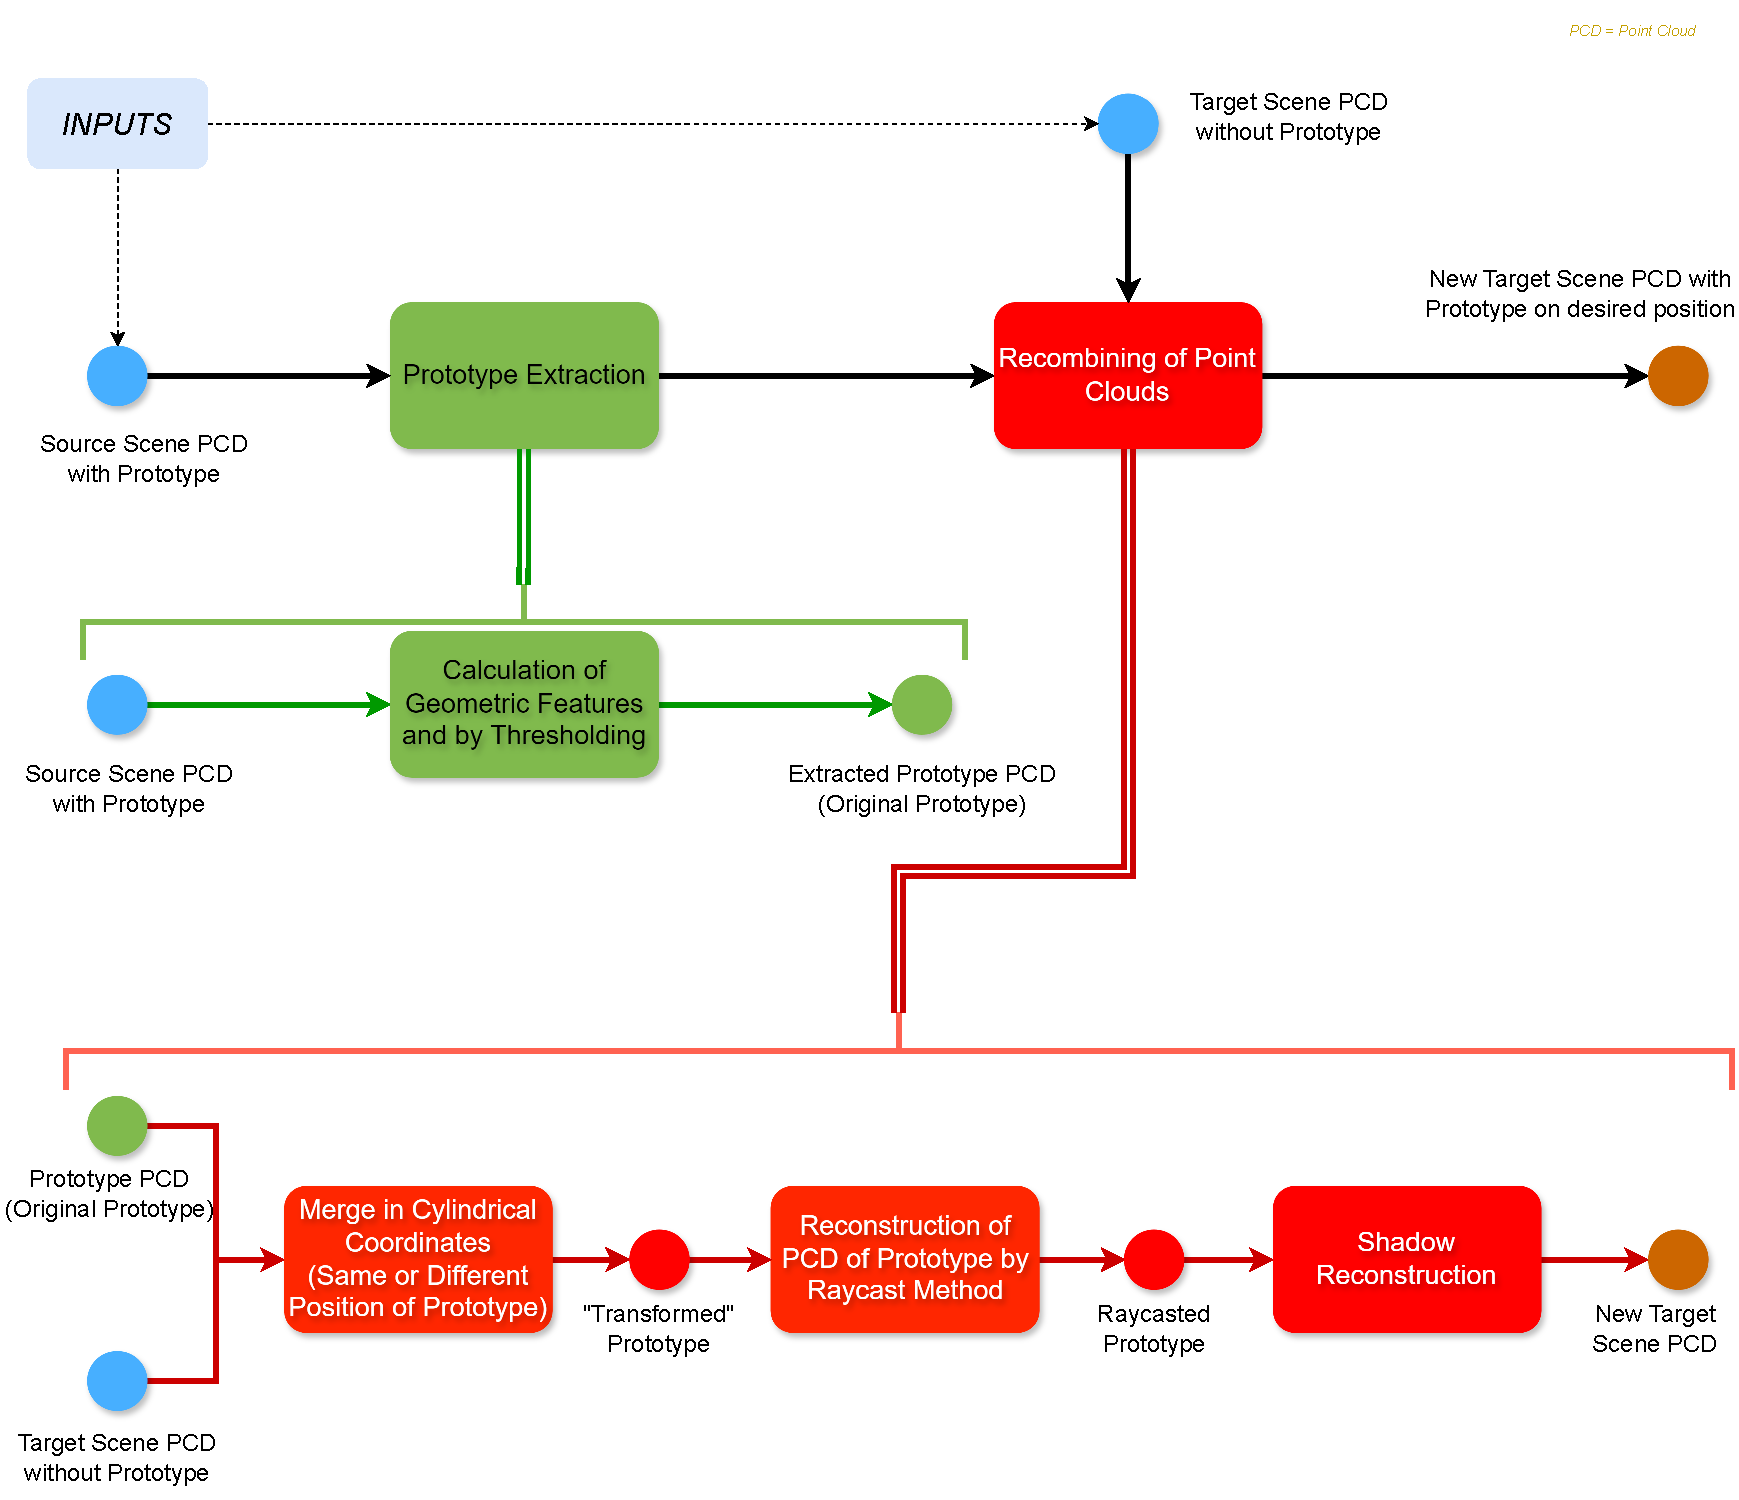
\includegraphics[width=1\linewidth]{97_graphics/concepts/graph_main.pdf}
    \caption{Concept graph representing the workflow of the project}
    \label{fig:concept-graph}
\end{figure}



\section{Prototype Extraction}
The thesis aim is to create new point clouds by extracting prototypes from one point cloud (source scene cloud) and placing the extracted prototype in a desired location on another point cloud (the target scene cloud). This facilitates the augmentation of an existing point cloud with additional objects or artifacts within the scene. Enabling such a process would increase the information content of the point cloud, which could be used to train various point cloud models or which could be used to test the feasibility of an autonomous driving system that would act when the prototypes are placed on the positions.
We have multiple options for prototype extractions from the source scene cloud. To extract the prototype from a source scene cloud, we first select a region of interest from where we need to extract the prototype. For our project, we had mainly three options of prototype extractions from the region of interest of the source scene cloud. 
\begin{enumerate}
    \item Extraction of a prototype using known Labels
    \item Extraction of a prototype using semantic \acrshort{ml} models
    \item Extraction of a prototype using geometric features
\end{enumerate}

\subsection{Extraction of prototype using known Labels}
Given a source scene cloud, a prototype could be extracted from a source scene cloud using the known labels of the point cloud. There is one precondition that needs to be met before using this approach. The precondition is that the point cloud from where the prototype is to be extracted should be labeled. Also, the label of the prototype to be extracted should be known. If we know the label of the prototype on a labeled point cloud then it would be straightforward and a perfect way to extract the prototype from the source scene. However, this is not always the case. Considering the time and cost effort required to get completely correct labeled data, most of the point cloud datasets available publicly online are just raw point clouds without labels. So choosing this approach is not feasible as a precondition has to be met before following this approach, which is not always the case. So we explored the next approach.

\subsection{Extraction of prototype using semantic ML models}
We also have an option of using state-of-the-art semantic models for the extraction of prototypes. A semantic model from \parencite{Chen2022} could be used to extract prototypes from the source scene cloud. The source scene cloud does not need to be labeled for the extraction of the prototype. However, one precondition has to be met to use \acrshort{ml} models for the prototype extraction. The ML model needs to be trained with the prototype-like objects and this requires a labeled dataset. Considering the laborious task of point cloud data annotations, we explored next on a simple yet effective approach to prototype extraction using geometric features.

\subsection{Extraction of prototype using geometric features}
Geometric features such as surface variation, planarity, linearity, etc are used for this step. We mainly focused on surface variation. Considering a part of the point cloud selected from a source scene, surface variation tells us the change in surface features for a selected neighborhood. Considering the goal of extracting a prototype from a region of interest, we mostly see an object standing on a flat surface. The roughness (surface variation) for the flat surface is low in comparison with the feature of the prototype to be extracted. This is because of the orientation of the points in the 3D space. Instead of calculating geometric features for a whole scene, we selected a region of interest where the prototype is located. Geometric features are calculated for the selected region of interest with appropriate parameters for the nearest neighbor search. Thus calculated geometric feature is filtered with appropriate values by trial and error. The result is an almost perfect extracted prototype. Thus we do not need to rely on known labels or on using \acrshort{sota} semantic 3d models for prototype extractions as for a selected \acrfull{roi}, just using the geometric features is also good enough. As a result, a prototype is extracted from the source scene cloud by thresholding the calculated geometric features. Thus extracted prototype will be combined with the target scene in the next step to generate a new scenario in the target scene cloud.

\section{Recombining of Point Clouds}
This step is represented by blocks with red color in the figure \ref{fig:concept-graph}. This stage involves the relocation of the prototype object to a specified target location within the target scene cloud. Subsequently, the point cloud associated with the prototype is recalculated based on its new position, followed by the computation of shadow casting generated by the transformed prototype. Each of these sub-steps can be described in detail below.

\subsection{Merge of Prototype and Target Scene Cloud}
The goal of this step is to place the extracted prototype on a selected region of the target scene cloud. Initially, experiments were done with registration algorithms like the \acrfull{icp} algorithm to find the optimal transformation of the prototype point cloud to the target location. This method proved to be ineffective, particularly in scenarios where we intend to relocate the prototype to a region within the target cloud characterized by sparse point density, such as areas distant from the origin of the point cloud. For the \acrshort{icp} algorithm to work, we need to have a set of correspondence between the points in the prototype cloud and the target scene cloud. Taking the lower points of the prototype (i.e. points with lower z-values) as correspondence points on the target region works with the ICP algorithm. But this step has a major drawback. This step assumes that the lower point(i.e. points with low z-values) of the prototype lies on the target region. This method fails to work if the point with lower z-values does not lie on the target location and is located slightly above the ground. This can be shown in the figure \ref{fig:icp_registration_analaysis}.

\begin{figure}[htbp]
    \centering
    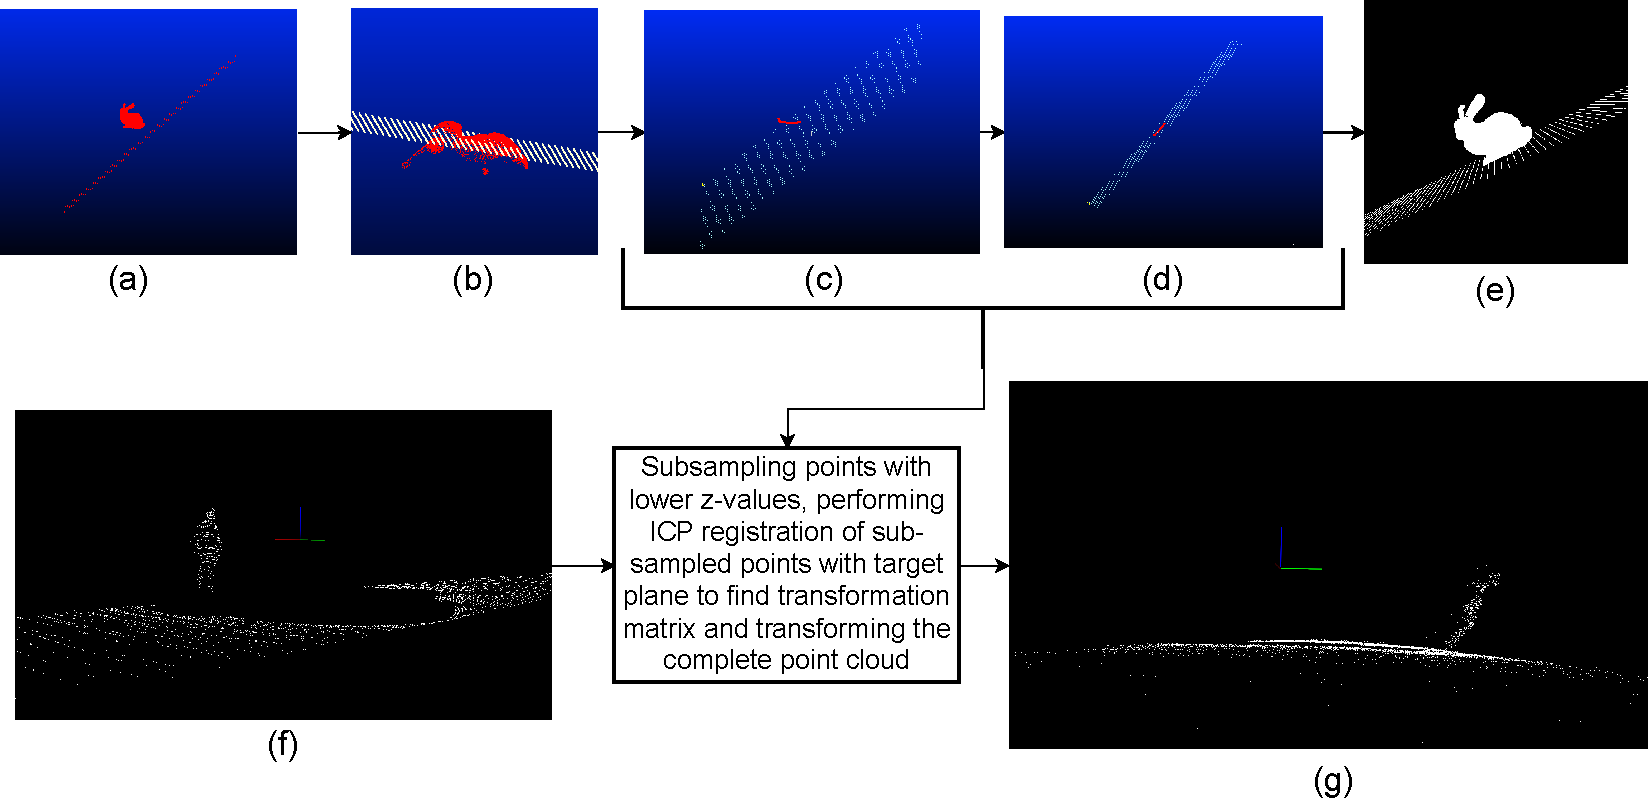
\includegraphics[width=1\linewidth]{97_graphics/concepts/icp_registration_analysis.pdf}
    \caption[Transformation of source cloud to target scene plane using \acrshort{icp} Registration Algorithm]{Transformation of source cloud to target scene plane using \acrshort{icp} Registration Algorithm (a)Bunny cloud needs to be placed on target inclined plane (b) Simple ICP registration with complete bunny cloud (c) Subsampling lower z-values points of bunny cloud (d) ICP registration of sampled points with the target plane (e) Bunny point cloud transformed using the transformation matrix calculated from subsampled ICP registration step (f) Point cloud of a person on a source scene (g) Point cloud of the person (inclined) after ICP registration on target scene cloud. } 
    \label{fig:icp_registration_analaysis}
\end{figure}


As shown in figure \ref{fig:icp_registration_analaysis}, even though the transformation of the bunny cloud to the inclined plane worked with some changes in the registration process, the transformation of the person's point cloud on the target scene did not work as expected. The vertically oriented person was transformed to a required location but the end result was that the person was inclined. This is because the points sub-sampled from the lower z-values of the person's point cloud did not lie on a horizontal plane. ICP registration worked on finding the minimum distance between the sub-sampled points and the target plane. Since the sub-sampled points do not lie on the same plane, the resulting transformation matrix resulted in the inclination of the person point cloud, even though the sub-sampled point cloud aligned perfectly on the target scene. So we approach a different methodology of transformation of the prototype to a desired location on a target scene. It can shown with a flow diagram using figure \ref{fig:prototype_transform_and_merge}

\begin{figure}[htbp]
    \centering
    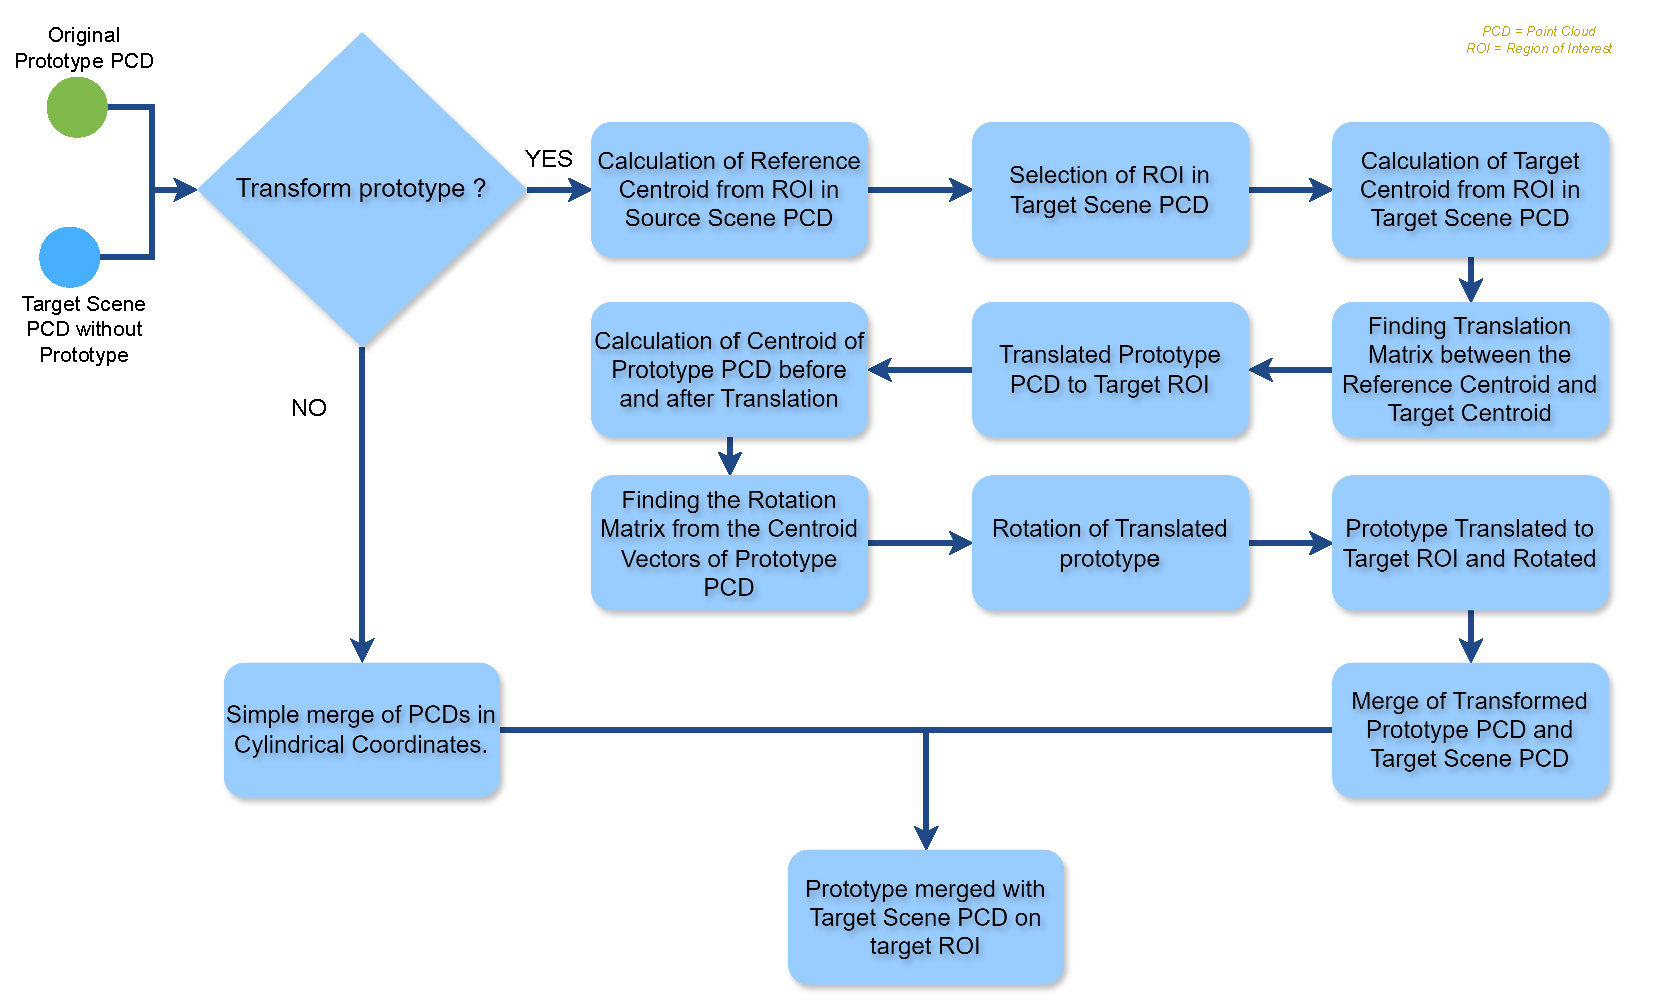
\includegraphics[width=1\linewidth]{97_graphics/concepts/prototype_extraction.pdf}
    \caption{Flowchart for the transformation of prototype cloud to target location and merge with target scene cloud}
    \label{fig:prototype_transform_and_merge}
\end{figure}

A simple geometrical approach is used for the transformation of the prototype to a region on the target scene cloud. If the prototype does not need to be transformed then it could be directly merged with the target scene and proceed with the next step. If the prototype needs to be transformed to a different location then first the centroid of reference is calculated from the region selected on the source scene cloud. This is calculated by adding all the points lying on the selected region on the source scene cloud that does not contain points from the prototype cloud. The resulting sum is divided by the total number of considered points to get the average value of the x, y, and z axis or the centroid of the ground plane. This calculation helps to get the orientation of the ground plane in the selected region of interest where the prototype is situated. Since the reference centroid is calculated from the points in the region of interest but excluding the prototype points, when performing this step, one needs to be careful so that no prototype points or high z-values points are considered for centroid calculation. Under such circumstances, the resulting centroid may not accurately represent the ground plane. Such a situation could lead to errors in the transformation process, potentially causing the prototype to be positioned above the ground plane in the designated region of the target scene cloud.

After the calculation of the reference centroid, a desired region of interest is selected on the target location, and the target centroid is calculated for the selected region. Using the two centroids, a translation matrix is created with which the prototype is translated to the target region in the target scene cloud. Using the vectors representing the reference centroid and target centroid, using equation \ref{eq:angle_between_vectors} the rotation matrix is calculated.

\begin{figure}[htbp]
    \centering
    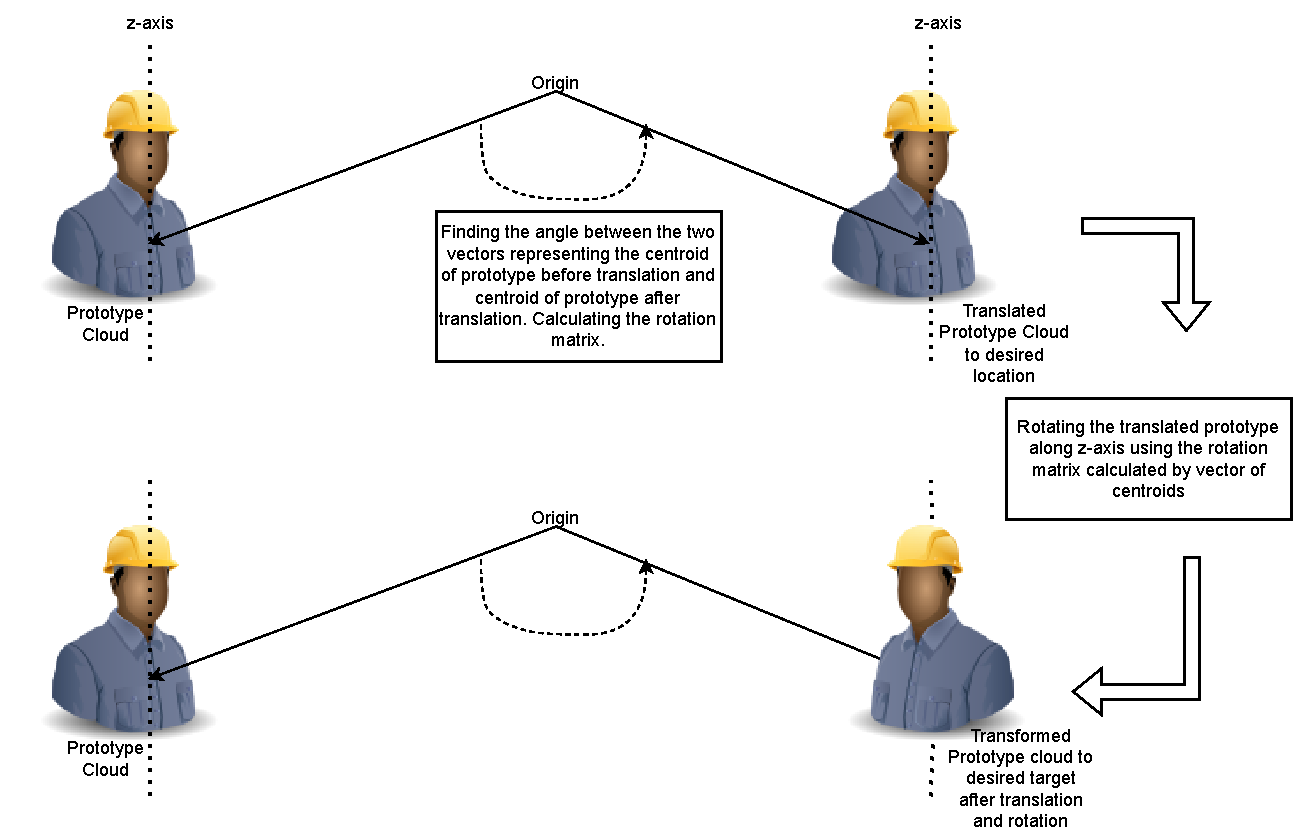
\includegraphics[width=1\linewidth]{97_graphics/concepts/rotational_matrix_calculation.pdf}
    \caption{Translation of Prototype, Calculation of Rotation Matrix and Rotation of Translated Prototype.}
    \label{fig:rotation_matrix_calculation}
\end{figure}

As shown in figure \ref{fig:rotation_matrix_calculation}, the calculated rotation matrix is then used to rotate the translated prototype cloud along the z-axis so that the transformed prototype object faces the origin. This is one of the most important steps. If the prototype is only translated to a desired location then the prototype might be facing in an incorrect direction (i.e. not viewing towards the origin). This false orientation of the prototype point cloud would result in a false calculation of points in the further steps as no points exist for surfaces that do not face the origin.

The transformed prototype cloud is then merged with the target scene cloud. The result is a prototype point cloud lying on top of the target region in the target scene cloud.


\subsection{Reconstruction of prototype point cloud on target scene cloud based on distance from the origin by Raycasting}

After the prototype point cloud has been placed in a target position on the target scene cloud, we need to find new point clouds of the prototype that accurately represent the prototype. We need to consider the following points for the reconstruction of points for the "transformed" prototype cloud.
\begin{itemize}
    \item Number of point cloud points for the prototype should vary based on distance from the origin.
    \item Need to consider the sparsity of points based on distance from the origin.
    \item New points representing the prototype surface should accurately represent the surface.
    \item Recalculated points should not be random. It should be a collection of points that follow the laser rays that originate from the origin in the target scene cloud.
\end{itemize}

In raycasting, a series of rays, originating from a viewpoint is passed to a certain distance. The point of intersection of rays to the obstacle is noticed. Based on the distance from the obstacle point, a 3D perspective is reconstructed in a 2D map for the viewpoint. Similar to such a principle, we cast rays to the target scene that contains the "transformed" prototype point cloud. But before the emission of rays, we reconstructed the surface of the "transformed" prototype cloud. We have options such as alpha shapes, ball pivoting, and poisson surface reconstructions that are used for the reconstruction of the surface from the point cloud. The poisson surface reconstruction method, as outlined by \parencite{kazhdan2006}, tackles the task of generating a smooth surface by addressing a regularized optimization problem. This approach contrasts with other methods that may yield less refined results, as they directly use the original points of the point cloud as the vertices of the resulting triangle mesh without any adjustments. Such reason leads us to use the poisson surface reconstruction for better construction of the surfaces. The Poisson surface reconstruction method extends its surface generation process to regions with sparse point density and even extrapolates into certain areas to create triangle meshes. The created triangle meshes also represent surfaces where there are minimum to no densities of points. To tackle such an issue, the reconstructed surface mesh is filtered. Filtering based on the density of the point also works but it requires manual setting of the threshold value. Instead of filtering by the density threshold value, triangles whose vertex do not contain the original point cloud points are removed. Following the later approach, no manual adjustment of the density threshold value is required.
After the surface mesh is filtered out and the resulting surface represents the mesh more accurately, rays are projected from the origin to a target region on the target cloud scene through the prototype surface mesh. To make the calculations faster, we select a region on the target scene cloud.

\begin{figure}[htbp]
    \centering
    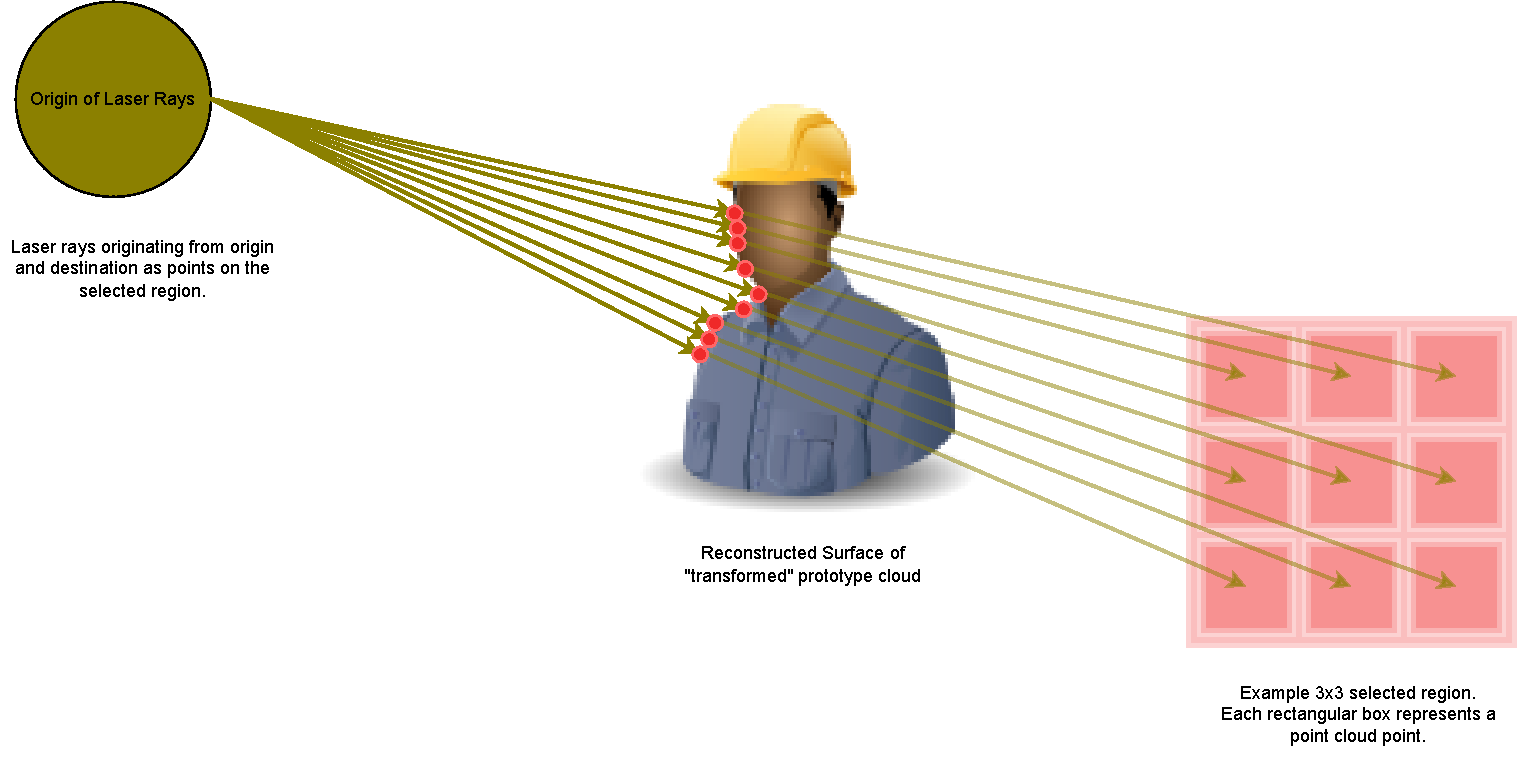
\includegraphics[width=1\linewidth]{97_graphics/concepts/raycasting.pdf}
    \caption{Rays traversing from the origin and terminating towards the selected points. Rays intersect with the reconstructed surface of the prototype, which is represented by red points}
    \label{fig:raycasting}
\end{figure}

As shown in figure \ref{fig:raycasting}, rays start from the origin and terminate at the selected region of interest. 3x3 rectangular box represents an example region that is selected on the target scene cloud. The region is selected in the target scene such that rays traversing from the origin to the designated points intersect the surface of the prototype(reconstructed surface after filtering by density).
Each 9 red box inside the selected region represents a point cloud. Thus in the example in figure \ref{fig:raycasting}, we are representing 9 points of a part of the selected target scene cloud. The rays travel toward the destination and some of the rays intersect the triangular mesh/surface of the prototype. Intersected point is calculated between the surface mesh and the casted rays. This intersected point gives us the new point cloud of the prototype. We call this new point cloud as Raycasted point cloud of prototype. This is represented by red points on the figure \ref{fig:raycasting}.

Two methods are explored for the calculation of the raycasted point cloud of the prototype. Since the reconstructed surface is represented by triangle mesh, when a single "laser beam" hits the surface of the prototype, it intersects with a triangle in the triangle mesh. 

\subsubsection{Calculation of Point based on Centroid of Triangle}

Figure \ref{fig:concept-raycasting_single_triangle_by_centroid} demonstrates a single ray originating from the origin and terminating at a point in the selected region of interest in the target scene cloud. The ray intersects the triangle mesh at (x, y, z). The vertex of the triangle is represented by (x0, y0, z0), (x1, y1, z1) and (x2, y2, z2). So to calculate the point (x, y, z), we calculate the centroid of the triangle mesh using equation \ref{equ:centroid_of_triangle}.

\begin{equation}
    \text{(x,y,z)} = \left( \frac{x0 + x1 + x2}{3}, \frac{y0 + y1 + y2}{3}, \frac{z0 + z1 + z2}{3} \right)
    \label{equ:centroid_of_triangle}
\end{equation}

These calculated points give us the raycasted point coordinates. This is represented by the red colored point in figure \ref{fig:concept-raycasting_single_triangle_by_centroid}. It can be viewed that the centroid of the point is not always the point of intersection. Here in the figure, the green point is the point of intersection to the triangle but this approach gives us the red color point. To reduce the errors, other methods are experimented.

\begin{figure}[htbp]
    \centering
    \begin{minipage}[b]{0.47\textwidth}
    \centering
    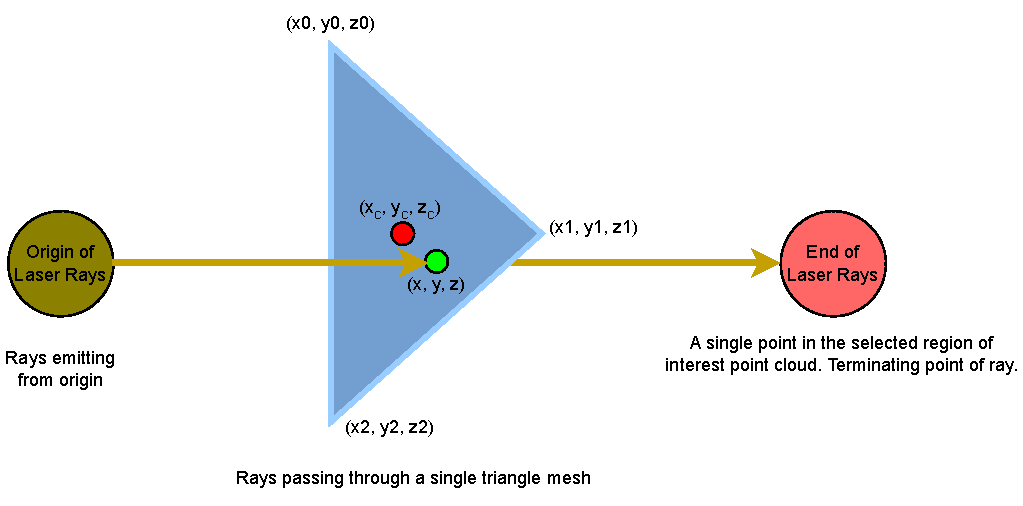
\includegraphics[width=1\linewidth]{97_graphics/concepts/raycasting_single_triangle_by_centroid.pdf}
    \caption{Calculation based on Centroid of the triangle.}
    \label{fig:concept-raycasting_single_triangle_by_centroid}
    \end{minipage}
    \hfill
    \begin{minipage}[b]{0.47\textwidth}
    \centering
    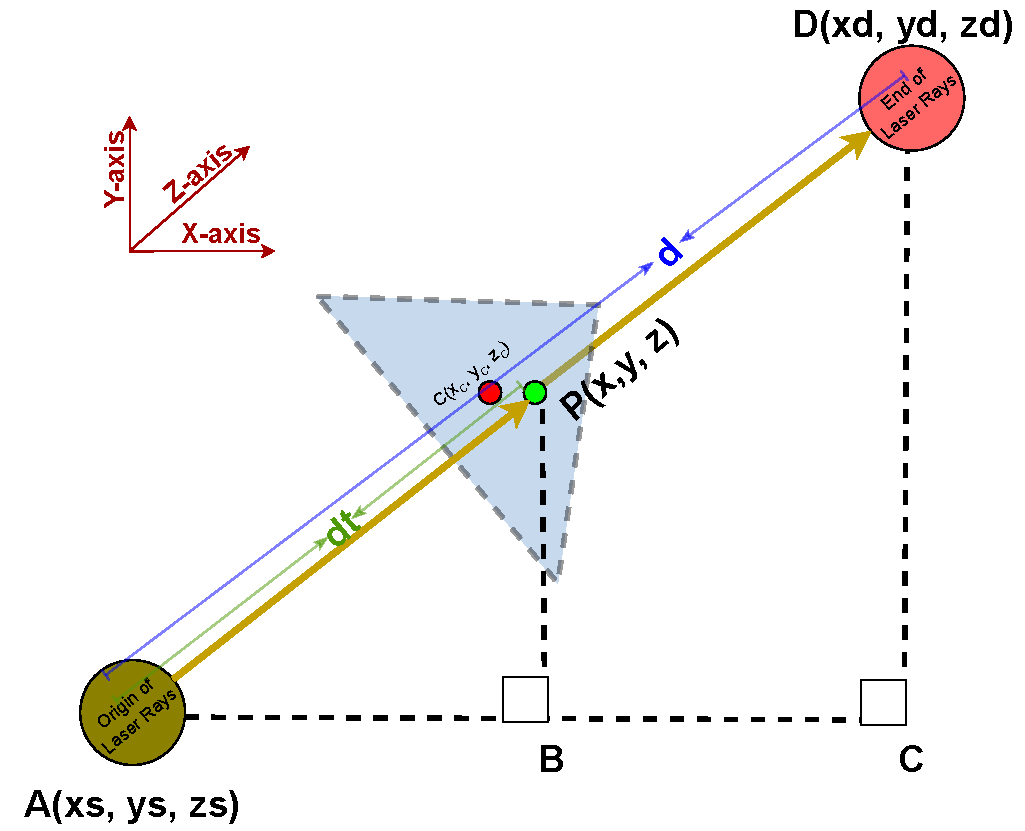
\includegraphics[width=1\linewidth]{97_graphics/concepts/raycasting_single_triangle_by_t_hit.pdf}
    \caption{Calculation based on hit distance to the triangle.}
    \label{fig:concept-raycasting_single_triangle_by_t_hit}
    \end{minipage}
\end{figure}

\subsubsection{Calculation of Point based on hit distance to the triangle mesh}
Using the centroid method to find the raycasted point is not always correct. The accuracy of the centroid method would depend on the number of triangles in the triangle mesh. The larger size of the triangle in the triangle mesh would result in a higher error rate. To eliminate such dependencies and error rates, the distance-based method is approached.  
In the figure \ref{fig:concept-raycasting_single_triangle_by_t_hit}, right-angle triangles are constructed. \(ABP\) represents the smaller triangle. \(ACD\) represents the larger triangle. \(dt\) represents the hit distance from the origin to the surface of the triangle. \(d\) represents the distance between the origin and the terminating point of the laser ray. Since two triangles are similar, using the law of similarity in triangles, we can write as follows : 

\begin{gather*}
\begin{aligned}
&\frac{AB}{AC} = \frac{AP}{AD} && \text{(Ratio of sides of triangle)}\hfill \\ \\
&\frac{x}{x_d} = \frac{d_t}{d} && \text{(Inserting length of the sides)}\hfill \\  \\
&x = x_d \times \frac{d_t}{d} && \text{(Result after Cross multiplication)}\hfill  \\  \\
\end{aligned}
\end{gather*}

\(X-axis\), \(Y-axis\), and \(Z-axis\) coordinates of the green color point can be obtained using the same approach.

\begin{equation}\label{eq:find_xyz}
    P(x, y, z) = \left( \: x_d \times \frac{d_t}{d}, \: y_d \times \frac{d_t}{d}, \: z_d \times \frac{d_t}{d} \: \right)
\end{equation}

% \begin{equation}\label{eq:find_y}
%     y = y_d \times \frac{d_t}{d}
% \end{equation}

% \begin{equation}\label{eq:find_z}
%     z = z_d \times \frac{d_t}{d}
% \end{equation}

\begin{equation}\label{eq:distance}
\text{distance(d)} = \sqrt{{(x_d - x_s)}^2 + {(y_d - y_s)}^2 + {(z_d - z_s)}^2}
\end{equation}

Equation \ref{eq:distance} represents the Euclidean distance between the two points in space (i.e. distance between vertex A and vertex D in figure \ref{fig:concept-raycasting_single_triangle_by_t_hit}). The \(d_t\) distance from the origin to the triangle can be obtained by raycasting. Hence, by using the equation \ref{eq:find_xyz} the coordinates of point \(P(x,y,z)\) can be calculated. This is represented by the green color point in figure \ref{fig:concept-raycasting_single_triangle_by_t_hit}. As shown in the figure, this point accurately represents the intersected point of the "laser ray" with a triangle mesh. For the calculation of the raycasted point cloud of the prototype, this approach is followed. As a final result, the raycasted point can be obtained which is represented by the red colored points in figure \ref{fig:raycasting}.

\subsection{Shadowcasting on the target scene cloud by Raycasted prototype cloud}

After the points of the prototype are recalculated based on the distance and orientation from the origin, we call the points raycasted points of the prototype. In the shadowcasting step, we reconstruct the shadow projected by the raycasted prototype on the target scene. Two methods for the calculation of shadow casting are experimented with. Two methods are the Hidden Point Removal (HPR) algorithm and calculation based on the Raycasted Rays.

% \begin{figure}[htbp]
%     \centering
%     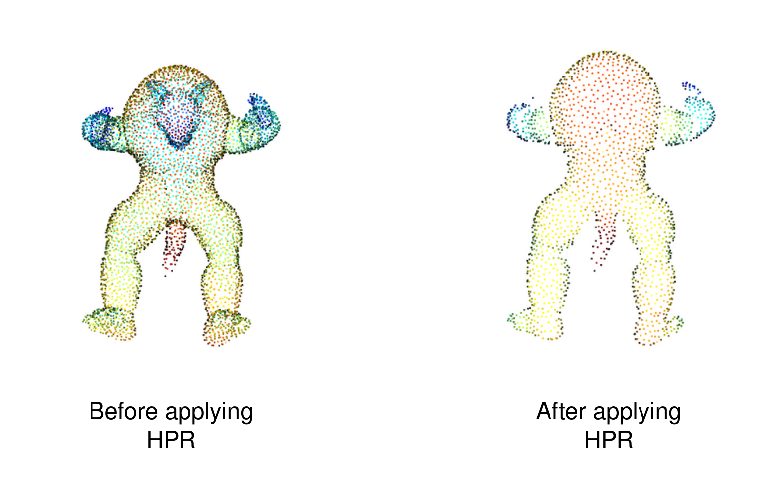
\includegraphics[width=0.5\linewidth]{97_graphics/concepts/shadowcasting_from_paper.pdf}
%     \caption{Point cloud of Armadilos: Left image represent point cloud of Armadilos without applying hidden point removal algorithm. Right image represent point cloud after applying hidden point removal algorithm. Source Open3d}
%     \label{fig:shadow_casting}
% \end{figure}

\subsubsection{Approach using HPR algorithm}
Based on a certain viewpoint in a point cloud, the HPR algorithm tells us if a point in the point cloud is hidden or visible. Consider an example as shown in figure \ref{fig:shadow_casting}. In the figure, the left image of Armadilos is shown without applying the HPR algorithm. The right image is shown after applying the HPR algorithm. In the figure \ref{fig:shadow_casting}, we could not distinguish if the left image of Armadilos is facing backward or frontwards (toward the direction of the reader). Since all the points are practically visible, the left image of the Armadillos in the figure seems to be facing backward and frontwards at the same time, creating confusion. After applying the HPR algorithm, the output is represented by the right side of the image in figure \ref{fig:shadow_casting}. We can clearly say that the Armadilo is facing backward with its back towards the reader. On applying the HPR, for the figure \ref{fig:shadow_casting}, the viewpoint is selected to be a point in the direction of the reader or outwards from the screen. This resulted in points being removed that are hidden from the viewpoint.

\begin{figure}[htbp]
    \centering
    \begin{minipage}[b]{0.45\textwidth}
    \centering
    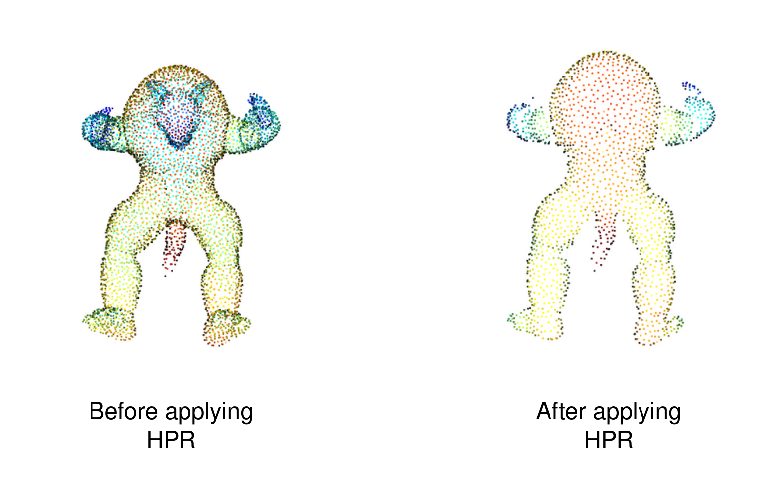
\includegraphics[width=0.5\linewidth]{97_graphics/concepts/shadowcasting_from_paper.pdf}
    \caption{Point cloud of Armadilos \parencite{open3d}}
    \label{fig:shadow_casting}
    \end{minipage}
    \hfill
    \begin{minipage}[b]{0.45\textwidth}
    \centering
    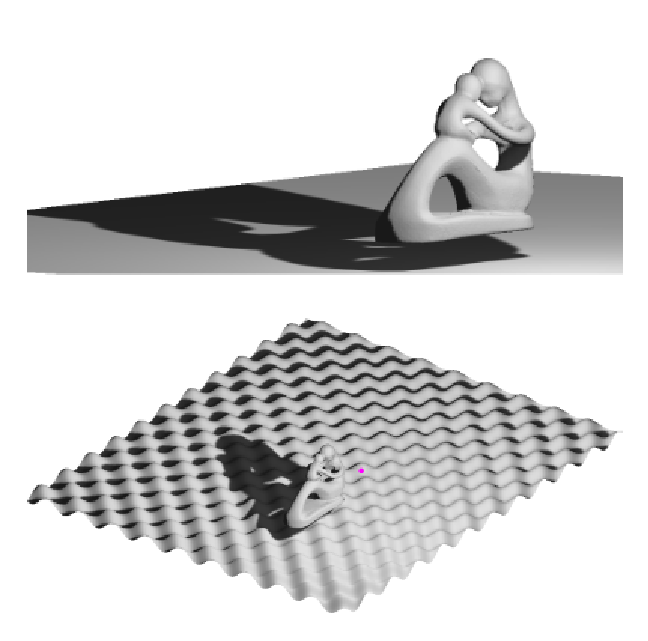
\includegraphics[width=0.5\linewidth]{97_graphics/concepts/hpr_reference_output.pdf}
    \caption{Shadow casting by HPR \parencite{katz2007}}
    \label{fig:hpr_reference_output}
    \end{minipage}
\end{figure}
% \begin{figure}[htbp]
%     \centering
%     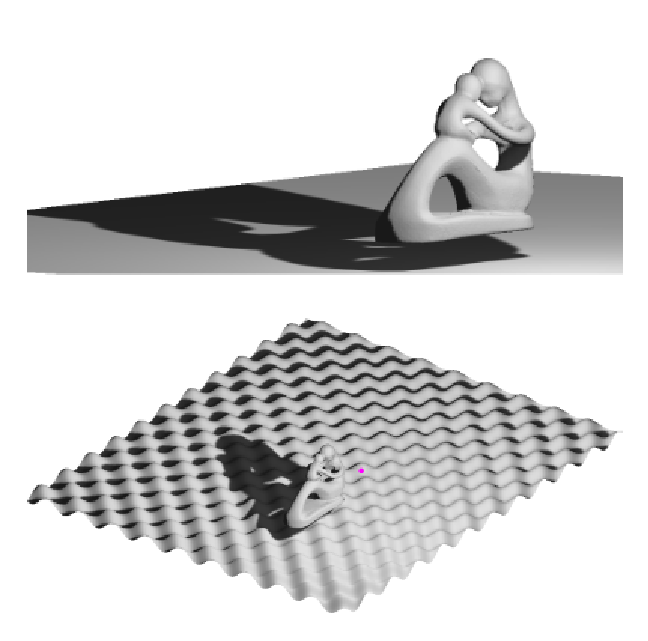
\includegraphics[width=0.5\linewidth]{97_graphics/concepts/hpr_reference_output.pdf}
%     \caption{Shadow casting by HPR algorithm on the target scene.\parencite{katz2007}}
%     \label{fig:hpr_reference_output}
% \end{figure}

In figure \ref{fig:hpr_reference_output}, the shadow is projected based on the visibility of points from the viewpoint. The viewpoint is defined by a pink color point on the bottom image of figure \ref{fig:hpr_reference_output}. Based on the visibility of the points from the viewpoint, the points are assigned low-intensity values or left unchanged. This resulted in the projection of shadow on the surface.
A similar principle is experimented for the casting of shadow by the raycasted point cloud on the target scene cloud. The viewpoint for HPR is set to the origin of the target scene point cloud. Instead of changing the intensity values of the hidden points, the points are removed from the point cloud and as a result, a shadow-projected target scene with raycasted prototype point cloud is received as output. 

\begin{figure}[htbp]
    \centering
    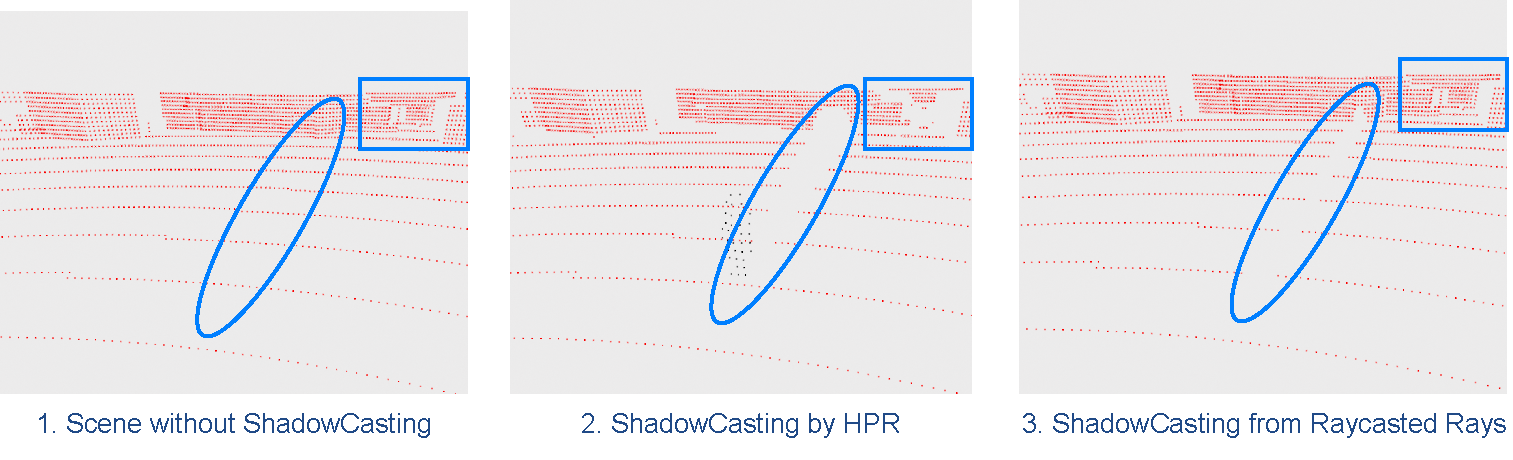
\includegraphics[width=0.9\linewidth]{97_graphics/concepts/shadow_casting_difference.pdf}
    \caption{Shadow Casting Difference between two methods}
    \label{fig:concept-shadow_casting_difference}
\end{figure}


\subsubsection{Approach using Raycasted Rays}
This approach is simple yet very effective. Instead of using the HPR algorithm for the calculation of shadow projection on the scene, the ray casted rays are considered for further calculations. Rays originate from the origin of the target scene point cloud and terminate at the points on the ROI in target scene cloud. Any rays intersecting the surface of the prototype give the raycasted point. Rays intersecting with the prototype surface means that the terminating point of the ray will be hidden by the surface of the prototype. Some rays do not intersect with the surface of the prototype. The terminating points of such rays are not hidden by the surface of the prototype. As a result, an accurate shadow of the prototype surface can be calculated. As shown in figure \ref{fig:concept-shadow_casting_difference}, this approach gives a perfect shadow of the reconstructed prototype surface. The blue rectangular box in the figure shows that applying the HPR algorithm affected the points that were not in the shadow region of the prototype. However, points not lying in the shadow region of the prototype were not affected using the raycasted method for shadow calculation. This approach is implemented for shadow calculation.
\begin{figure}[htbp]
    \centering
    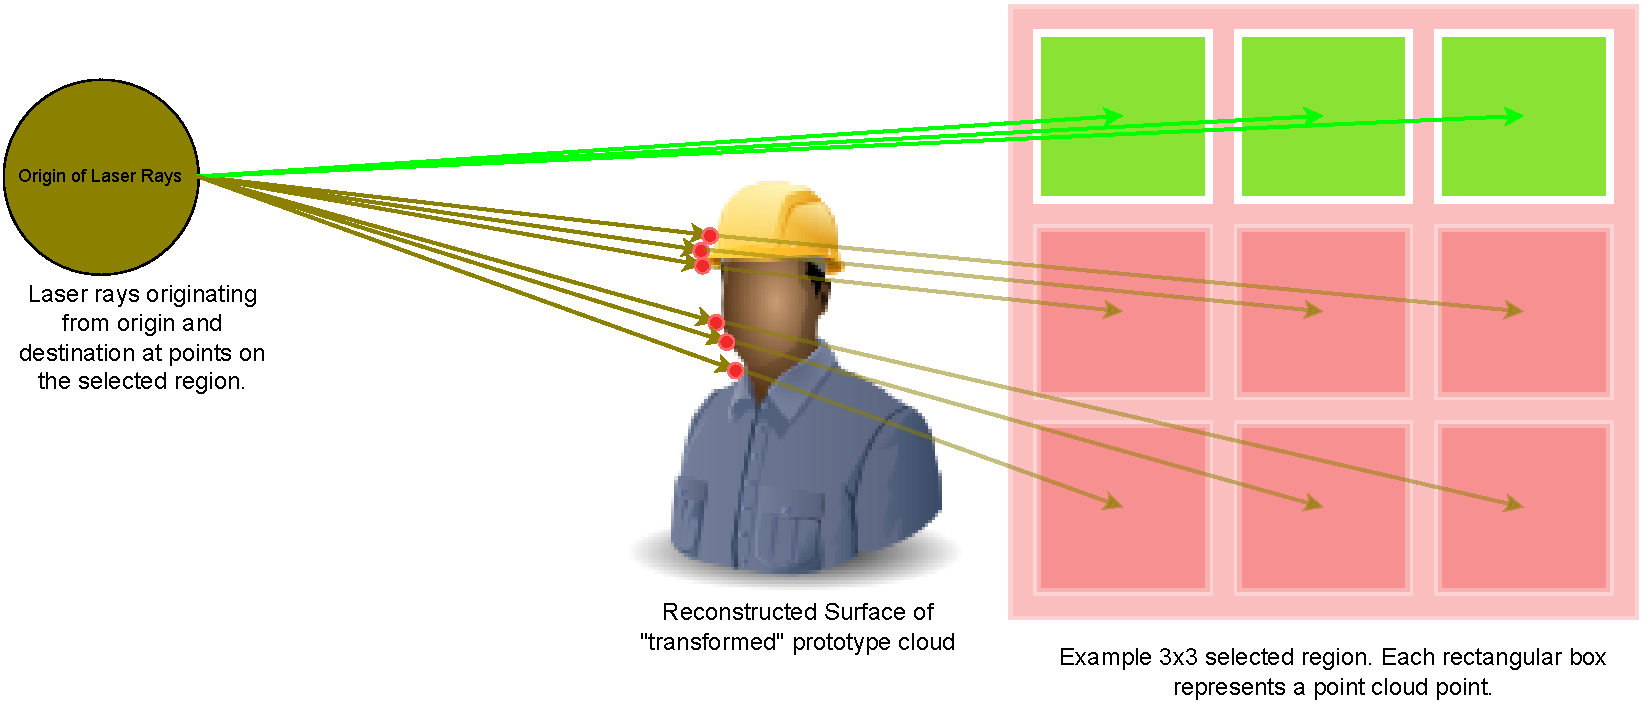
\includegraphics[width=0.9\linewidth]{97_graphics/concepts/shadow_casting_by_raycast_method.pdf}
    \caption{Shadow Casting Approach using Raycasted Rays}
    \label{fig:concept-shadow_casting_by_raycast_method}
\end{figure}

Figure \ref{fig:concept-shadow_casting_by_raycast_method} shows an example of shadow casting on the target region. The green-colored rays, originating from the origin to the point in the selected region, were not intersected with the prototype surface represented by triangle mesh. So the terminating points of the green colored rays are not hidden from the origin. This is represented by the green-colored square on the figure. The red-colored square represents that the point is hidden by the surface. The rays that originate from the origin designated to the red-colored square are blocked by the surface of the prototype. The intersected point of the rays with the surface is represented by red-colored points and is called the raycasted points. The terminating point of the rays blocked by the surface or prototype is the shadowed region.

\section{Functional Description of the implementation}

Figure \ref{fig:functional_description_of_concept} shows an example of high-level implementation details of the project. The images present in the top row of the figure \ref{fig:functional_description_of_concept} represent scenes. The top left image represents a source scene. A prototype (person) is present on the scene, which is represented in the red rectangular box. The top middle image of the figure represents a target scene. The goal of the project is to extract a person from the source scene and insert the extracted person into the target scene. This results in a new scene. In the figure, the target scene is modified in such a way that a person is now present on the target scene. So the recombination between the two upper left scenes would result in a new scene similar to the top right of the figure \ref{fig:functional_description_of_concept}.
These different scenes were captured in the \acrfull{carla} simulator \parencite{Dosovitskiy17}. An ego vehicle was summoned on CARLA using carla-ros-bridge. The prototype or person was summoned to a specified location near the ego vehicle.

\begin{figure}[htbp]
    \centering
    \includegraphics[width=1\linewidth]{97_graphics/concepts/functional_description_of_concept.pdf}
    \caption{Functional description of the implementation}
    \label{fig:functional_description_of_concept}
\end{figure}

\section{Technical Description of the implementation}
The aim of the project is the creation of a new scene. This project works on the point cloud level. Functional description of the projects shows a higher level overview of the project using images from \acrshort{carla}. This section describes the technical aspects of the project. The point cloud images shown on the top row in figure \ref{fig:technical_description_of_implementation} correspond to the point cloud of scenes represented by the top row images in figure \ref{fig:functional_description_of_concept}. The ego vehicle is attached with a lidar sensor, which gives a lidar point cloud of the current scene continuously. The point cloud data is made available to \acrfull{ros} topic by carla-ros-bridge, which is then captured by written scripts. 

\begin{figure}[htbp]
    \centering
    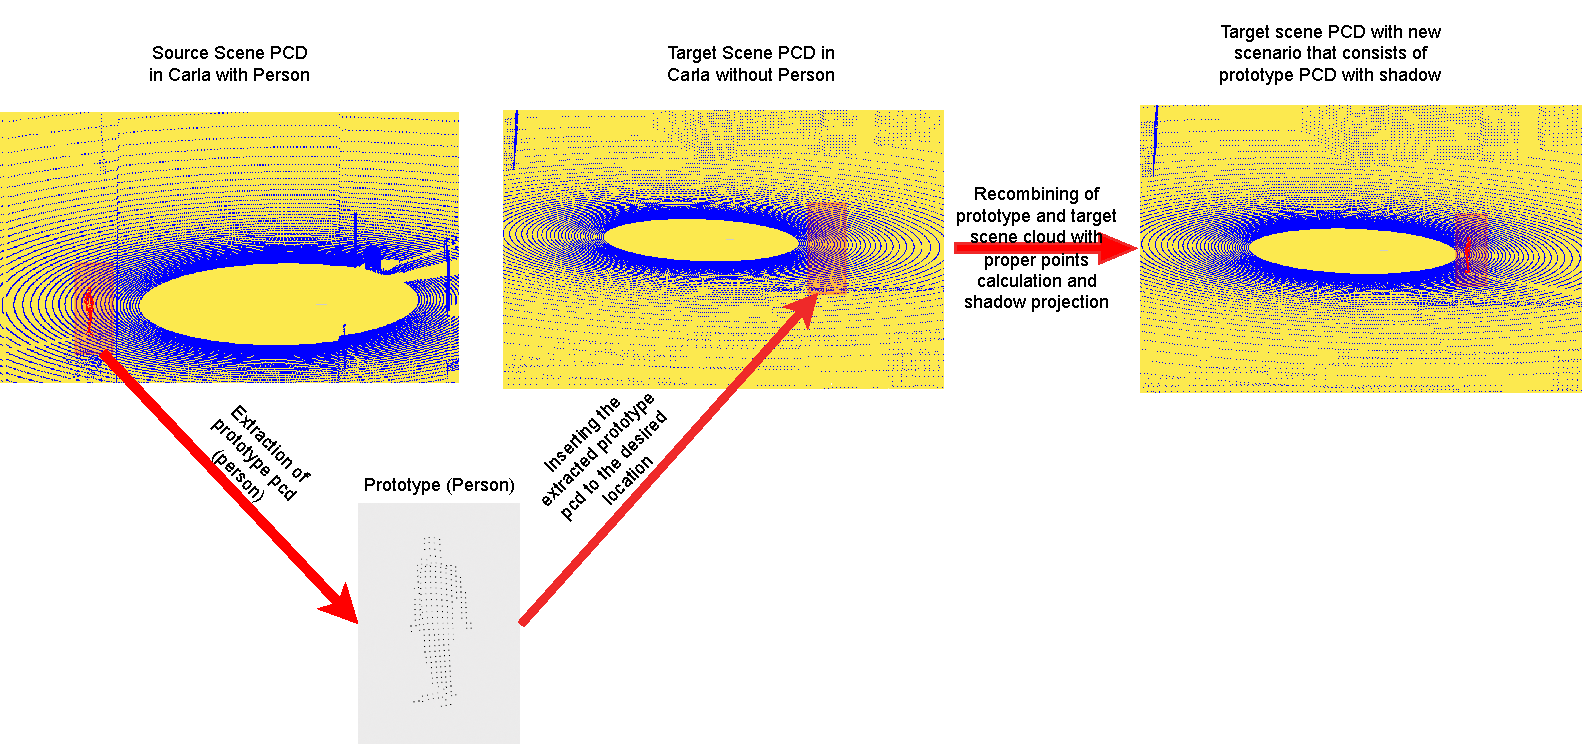
\includegraphics[width=1\linewidth]{97_graphics/concepts/technical_description_of_concept.pdf}
    \caption{Technical description of the implementation}
    \label{fig:technical_description_of_implementation}
\end{figure}

The image on the top row leftmost side in figure \ref{fig:technical_description_of_implementation} represents a source scene cloud. The task of the project is to extract the prototype cloud from the source scene cloud. The prototype cloud is represented by red colored points on the source scene cloud. The prototype point cloud is to be extracted using the geometric features of the point cloud. The region of interest from where we would like to extract a prototype is represented by a red rectangular box in all the top row images in figure \ref{fig:technical_description_of_implementation}. In the source scene cloud, geometric features on the selected region of interest are calculated. The separation of the prototype point cloud from the target scene is done by thresholding the geometric features. This gives us an extracted prototype cloud represented by the image on the bottom row of figure \ref{fig:technical_description_of_implementation}. This prototype needs to be placed on the target scene region of interest in the top row middle image of the same figure. With the proper transformation of the prototype cloud according to the geometry of the target scene cloud, the prototype is placed and the projected shadow is calculated. A final output point cloud is created by combining the prototype from the source scene cloud into the target scene cloud. This new point cloud is represented by the top row rightmost image in the figure \ref{fig:technical_description_of_implementation}.
